\chapter{Esperimenti}\label{esperimenti}
In questo capitolo verranno presentati i test condotti sulle performance del sistema di \emph{Assurance Engine} collegato ad Elasticsearch.
L'obiettivo è quello di descrivere i tipi di test/benchmark eseguiti e i risultati oggettivi ottenuti tramite grafici e tabelle riepilogative.
Questi benchmark sono stati selezionati perché rappresentano i principali casi d'uso nel contesto di misurazione e valutazione delle performance.
In altre parole, sono stati analizzati quegli aspetti statistici chiave, cruciali per comprendere e ottimizzare le prestazioni complessive del sistema.
I benchmark sono stati condotti utilizzando Criterion\footnote{\url{https://bheisler.github.io/criterion.rs/book/}}, una libreria di benchmarking utilizzata per misurare e analizzare prestazioni di esecuzione di specifiche funzioni per il linguaggio di programmazione Rust.

%%%%%%%%%%%%%%%%%%%%%%%%%%%%%%%%%%%%%%%%%%%%%%%%%%%%%%%%%%%%
%%%%%%%%%%%%%%%%%%%%%%%%%%%%%%%%%%%%%%%%%%%%%%%%%%%%%%%%%%%%
\section{Statistiche offerte}
L'implementazione di benchmark tramite Criterion fornisce delle tabelle, denominate \textit{additional statistics}, e dei diagrammi per poter analizzare e confrontare i risultati ottenuti.
Vengono elencate di seguito tutte le \textit{additional statistics} ottenibili con una breve illustrazione. \'E da considerare che tutte le valutazioni vengono espresse tramite intervalli di confidenza, seguono quindi la forma \texttt{[<lower bound> <estimated>  <upper bound>]}.
%https://bheisler.github.io/criterion.rs/book/user_guide/command_line_output.html#additional-statistics
\begin{itemize}
	\item \textbf{R2} Coefficiente di Determinazione. \'E una misura della bontà di adattamento di un modello di regressione lineare ai dati; misura quindi la correttezza del modello statistico utilizzato. Se il valore R2 è basso, questo potrebbe indicare che il benchmark non sta eseguendo la stessa quantità di lavoro a ogni iterazione.

	\item \textbf{Mean} Media dei tempi per iterazione
	\item \textbf{Std. Dev.} Deviazione Standard dei tempi per iterazione. \'E una misura della dispersione o variabilità di un insieme di dati che indica quanto i valori di un dataset si discostano in media dalla loro media aritmetica. \\
	      Se è più grande rispetto agli altri valori di tempo significa che i benchmark sono rumorosi e potrebbe essere necessario modificarli per ridurre il rumore.

	\item \textbf{Median} Mediana. \'E una misura che indica il valore centrale di una distribuzione; divide un dataset ordinato in due metà uguali contenenti lo stesso numero di valori (o quasi).
	\item \textbf{\gls{MAD}} Deviazione Assoluta Mediana. \'E una misura di dispersione che quantifica quanto i dati si discostano dalla loro mediana. \'E un'alternativa alla deviazione standard e viene utilizzata per misurare la variabilità dei dati in modo che sia meno influenzata dai valori estremi o outliers. \\
	      Se la deviazione assoluta mediana è ampia indica che i parametri di riferimento sono rumorosi.

	\item \textbf{Outliers} Valori anomali. Vengono rilevate misurazioni insolitamente sproporzionate rispetto alle restanti, sia valori troppo alti che troppo bassi. \\
	      Se sono presenti molti valori anomali, la misurazione ci suggerisce che i risultati del benchmark sono rumorosi e non pienamente affidabili.
\end{itemize}


Oltre ai dati presentati in forma tabellare (ed immagazzinati in formato JSON), Criterion mette a disposizione vari diagrammi o \textit{plot} per rappresentare graficamente le performance.

\begin{itemize}
	\item \textbf{Violin plot} Diagramma a violino. Una rappresentazione statistica che descrive distribuzioni di probabilità utilizzando curve di densità; viene utilizzato per confrontare distribuzioni e quindi confrontare i benchmark.
	\item \textbf{Density plot} Diagramma della densità. Mostra il tempo medio per iterazione. Nel diagramma si ha una regione colorata che rappresenta la probabilità che un iterazione richieda quella quantità di tempo e una linea marcata che identifica la media.
	\item \textbf{Time/Iteration plot} Mostra il tempo medio di iterazione impiegato dai diversi sample o tentativi. Ogni tentativo (generalmente da 0 a 100) viene rappresentato da un puntino e l'altezza ne definisce il tempo utilizzato.
\end{itemize}

%%%%%%%%%%%%%%%%%%%%%%%%%%%%%%%%%%%%%%%%%%%%%%%%%%%%%%%%%%%%
%%%%%%%%%%%%%%%%%%%%%%%%%%%%%%%%%%%%%%%%%%%%%%%%%%%%%%%%%%%%
\section{Benchmark}
I benchmark scritti utilizzando il framework Criterion vengono eseguiti tramite il comando \texttt{cargo bench -p ae-probes --bench elastic\_probes}.
L'esecuzione di ogni benchmark viene suddivisa in quattro fasi.
\begin{enumerate}
	\item \textit{\textbf{Warm-up}}: la funzione sottoposta al benchmark viene eseguita ripetutamente per un periodo di tempo configurabile, di default 3 secondi.
	      Serve a riscaldare le cache del processore e (se applicabile) le cache del file system per adattarsi al nuovo carico di lavoro.

	\item \textit{\textbf{Measurement}}: la funzione sottoposta al benchmark viene eseguita ripetutamente per generare una stima del tempo impiegato da ogni iterazione; ogni iterazione viene definite come un sample e contiene le rispettive misurazioni.

	\item \textit{\textbf{Analysis}}: i sample vengono analizzati per calcolare le statistiche che vengono riportate, salvate e disegnate.

	\item \textit{\textbf{Comparison}}: il sample corrente viene confrontato con il sample ottenuto nell'iterazione del benchmark precedente.
\end{enumerate}

Terminate queste fasi e quindi terminato il benchmark viene generata una struttura di directory all'interno del progetto Rust sotto \textit{assurance-engine/target/criterion/<BENCHMARK\_NAME>} come mostrato nella Figura \ref{benchmark directory}.

\begin{figure}
	\centering
	\begin{subfigure}{\textwidth}
		\dirtree{%
			.1 \textbf{BENCHMARK\_NAME/}.
			.2 \textbf{base/}.
			.3 benchmark.json.
			.3 estimates.json.
			.3 sample.json.
			.3 tukey.json.
			.2 \textbf{change/}.
			.3 estimates.json.
			.2 \textbf{new/}.
			.3 benchmark.json.
			.3 estimates.json.
			.3 sample.json.
			.3 tukey.json.
			.2 \textbf{report/}.
			.3 both/.
			.4 pdf.svg.
			.4 iteration\_times.svg.
			.4 regression.svg (optional -> not present).
			.3 change/.
			.4 mean.svg.
			.4 median.svg.
			.4 t-test.svg.
			.3 index.html.
			.3 MAD.svg.
			.3 mean.svg.
			.3 median.svg.
			.3 SD.svg.
			.3 slope.svg (optional -> not present).
			.3 pdf.svg.
			.3 pdf\_small.svg.
			.3 relative\_pdf\_small.svg.
			.3 iteration\_times.svg (optional -> present).
			.3 iteration\_times\_small.svg (optional -> present).
			.3 relative\_iteration\_times\_small.svg (optional -> present).
			.3 regression.svg (optional -> not present).
			.3 regression\_small.svg (optional -> not present).
			.3 relative\_regression\_small.svg (optional -> not present).
		}
	\end{subfigure}
	\caption{Directory tree generato dai benchmark di Criterion}\label{benchmark directory}
\end{figure}

La cartella \textit{/new} contiene le statistiche dell'ultimo benchmark eseguito mentre la cartella \textit{/base} include le statistiche del benchmark precedente oppure è rimpiazzata da cartelle con il nome dei benchmark salvati.
Tramite il comando \texttt{cargo bench -\phantom{}-bench elastic\_probes -\phantom{}- -\phantom{}-save-baseline <nome>} è possibile andare a salvare un benchmark con un nome e
tramite il comando \texttt{cargo bench -\phantom{}-bench elastic\_probes -\phantom{}-baseline <nome>} è possibile selezionarlo come benchmark per il confronto. \'E stato salvato un benchmark eseguito localmente nel laboratorio.\\
Il comando utilizzato per ottenere le statistiche dettagliate delle valutazioni in locale e confrontarle graficamente coon le altre salvate precedentemente è il seguente: \texttt{cargo bench -p ae-elastic-probe -\phantom{}-bench elastic\_probes -\phantom{}- -\phantom{}-load-baseline locale -\phantom{}-baseline old}. \\
La cartella \textit{/report} contiene tutti i diagrammi, sia quelli generati del singolo benchmark che quelli del confronto con uno precedente, contenuti nella sotto-cartella \textit{/both}.
I risultati tramite interfaccia grafica sono consultabili aprendo il file \textit{/report/index.html}.

Il benchmark effettuato valuta concretamente l'esecuzione di 4 funzione suddivise a coppie. Le prime due utilizzano la ricerca tramite Query \gls{DSL} proposta nel Codice \ref{JSON query all} che estrae tutti gli elementi e li ordina cronologicamente. Le altre due, invece, utilizzano la ricerca tramite query SQL proposta nel Codice \ref{JSON query sql} che estrae due campi dall'indice filtrando sulla data. Ogni coppia è costituita da una funzione \texttt{measure()} per le Metriche e da una funzione \texttt{evaluate()} per i Contratti. \\
Di seguito, per ogni tipo di ricerca (SEARCH e SQL), viene proposto prima un confronto tra l'esecuzione dei due metodi, \texttt{measure} ed \texttt{evaluate}, tramite un diagramma a violino e poi un'analisi dettagliata dei metodi presi singolarmente.

%%%%%%%%%%%%%%%%%%%%%%%%%%%%%%%%%%%%%%%%%%%%%%%%%%%%%%%%%%%%
%%%%%%%%%%%%%%%%%%%%%%%%%%%%%%%%%%%%%%%%%%%%%%%%%%%%%%%%%%%%
\section{SEARCH Benchmark}
Benchmark effettuato sulle funzioni \texttt{measure()} ed \texttt{evaluate()} basate sulla Query \gls{DSL} proposta nel Codice \ref{JSON query all} che estrae tutti gli elementi e li ordina cronologicamente.

\paragraph{Confronto funzioni benchate}
La Figura \ref{violino search} mostra due distribuzioni di probabilità indicanti il tempo medio di esecuzione delle funzioni \texttt{evaluate} e \texttt{measure}.
L'asse delle ascisse rappresenta il tempo di esecuzione, mentre quello delle ordinate i due benchmark da confrontare.
Si osserva come le distribuzioni si concentrino introno al valore medio, 6 ms per le metriche e 5 ms per i contratti. 
Tuttavia, si nota come l'ampiezza del benchmark di Metric si discosti notevolmente dal valore medio a causa di alcuni \textit{outliers} misurati, sopra i 9 ms; sono identificati da una riga orizzontale che quindi ne definisce una probabilità trascurabile.
In conclusione, l'esecuzione del benchmark sui contratti è stata omogenea in quanto tutte le misurazioni hanno ottenuto valori addensati intorno ai 5 ms. Nel caso dei benchmark sulle metriche, invece, si nota una media spostata leggermente verso destra, 6 ms, poiché influenzata da misurazioni outliers.

\begin{figure}[h]
	\centering
	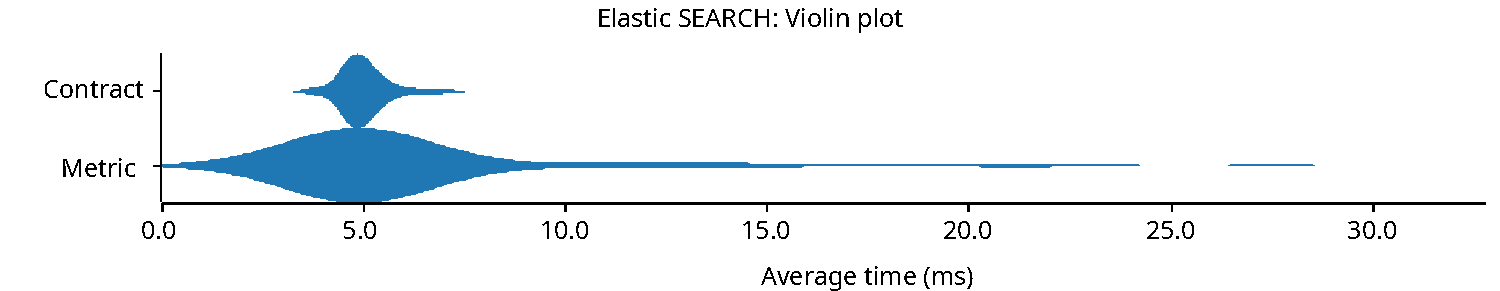
\includegraphics[width=1\linewidth]{images/benchmark/SEARCH/search-violin.pdf}
	\caption{Diagramma a violino richieste di tipo SEARCH}\label{violino search}
\end{figure}
%%%%%%%%%%%%%%%%%%%%%%%%%%%%%%%%%%%%%%%%%%%%%%%%%%%%%%%%%%%%
%%%%%%%%%%%%%%%%%%%%%%%%%%%%%%%%%%%%%%%%%%%%%%%%%%%%%%%%%%%%
\subsection{Metric - \texttt{measure()}}\label{section metric search}
\paragraph{Diagramma distribuzione probabilità-tempo}
La Figura \ref{densità metric search} illustra la distribuzione di probabilità relativa al tempo necessario per eseguire il metodo \texttt{measure}. Si possono osservare quattro picchi nel diagramma. 
Il primo, nonché più significativo, determina prevalentemente il comportamento di questa distribuzione, in quanto possiede l'altezza massima e quindi una densità di probabilità maggiore; il picco si trova sul valore 5 ms.
Gli altri altri 3 picchi identificati sono di rilevanza inferiore più ci si allontana dal valore del picco massimo. 
Questi ultimi si trovano oltre al valore definito come limite massimo per decretare un valore conforme agli altri e quindi non outlier; nel diagramma viene rappresentato da una linea rossa a 9 ms, ``severe outliers''. Gli outlier sono identificati da puntini rossi mentre la media è rappresentata da una linea blu a a 6.2 ms.
\begin{figure}[h]
	\centering
	
\includegraphics[width=1\linewidth]{images/benchmark/SEARCH/metric/density.pdf}
	\caption{Diagramma densità probabilistica richieste \texttt{measure} di tipo SEARCH}\label{densità metric search}
\end{figure}

\paragraph{Statistiche calcolate}
Nella Tabella \ref{benchmark search metric} vengono mostrate le statistiche ottenute tramite i benchmark. Si nota una media del tempo di esecuzione pari a 6.2 ms e una deviazione standard rispetto tale valore pari a 4.1 ms.
\begin{table}[h]
	\caption{Valutazioni statistiche SEARCH/Metric benchmark}\label{benchmark search metric}
	\centering
	\begin{tabularx} {0.9\textwidth}
		{C| c*{3}{C}} % C è un column type definito nel main
		\toprule
		\textbf{Misurazione} & \textit{Lower bound} & \textbf{Estimate}  & \textit{Upper bound} \\

		\midrule
		\textbf{Mean}        & 5.5126 ms            & \textbf{6.2485 ms} & 7.1098 ms            \\
		\textbf{Std. Dev.}   & 2.5683 ms            & \textbf{4.1361ms}  & 5.4378 ms            \\
		\textbf{Median}      & 4.8315 ms            & \textbf{5.0052 ms} & 5.1727 ms            \\
		\textbf{\gls{MAD}}   & 691.05 µs            & \textbf{906.15 µs} & 1.0739 ms            \\
		\textbf{R2}          & 0.0005357            & \textbf{0.0005529} & 0.0005297            \\

		\bottomrule
	\end{tabularx}
\end{table}

\paragraph{Diagramma Sample-Time}
La Figura \ref{iter-time metric search} rappresenta un diagramma che mostra il tempo che ogni sample ha impiegato per terminare l'esecuzione della funzione. Sono presenti 100 sample e l'altezza ne indica il tempo impiegato. Si nota come le prime 14 iterazioni hanno tempi maggiori o uguali ai 10 ms e quindi, essendo maggiori della soglia di normalità (9 ms), vengono identificati come outliers. Le iterazioni successive si stabilizzano introno ai 5 ms.
\begin{figure}[h]
	\centering
	
\includegraphics[width=1\linewidth]{images/benchmark/SEARCH/metric/iteration-times.pdf}
	\caption{Diagramma iteration/time richieste \texttt{measure} di tipo SEARCH}\label{iter-time metric search}
\end{figure}

%%%%%%%%%%%%%%%%%%%%%%%%%%%%%%%%%%%%%%%%%%%%%%%%%%%%%%%%%%%%
%%%%%%%%%%%%%%%%%%%%%%%%%%%%%%%%%%%%%%%%%%%%%%%%%%%%%%%%%%%%
\subsection{Contract - \texttt{evaluate()}}\label{section contract search}
\paragraph{Diagramma distribuzione probabilità-tempo}
La Figura \ref{densità contract search} presenta la distribuzione di probabilità del tempo di esecuzione del metodo \texttt{evaluate}.
Si nota la presenza di un singolo picco centrale che si discosta leggermente dalla media, il cui valore è 5 ms. 
Questo scostamento è causato dalla presenza di alcuni outliers lievi, che si trovano oltre i 6.1 ms e influenzano leggermente la valutazione finale. La concentrazione massima di densità risiede tra i valori temporali 4.5 e 5.5.
\begin{figure}[H]
	\centering
	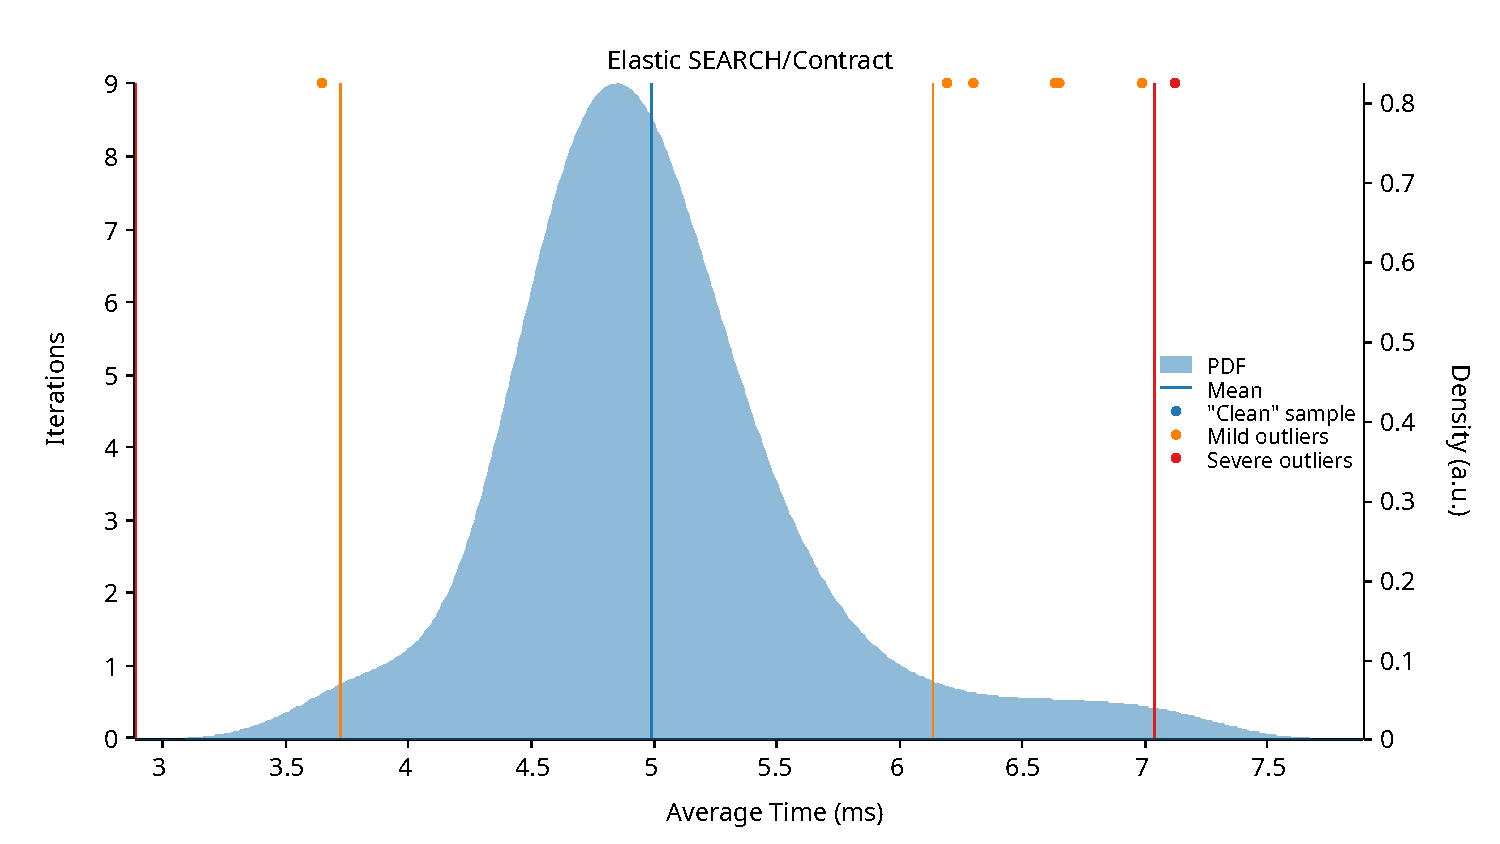
\includegraphics[width=1\linewidth]{images/benchmark/SEARCH/contract/density.pdf}
	\caption{Diagramma densità probabilistica richieste \texttt{evaluate} di tipo SEARCH}\label{densità contract search}
\end{figure}

\paragraph{Statistiche calcolate}
La Tabella \ref{benchmark search contract} riporta le statistiche derivanti dai benchmark. Si evidenzia un tempo medio di esecuzione pari a 4.9 ms e una deviazione standard pari a 600.06 µs, il che indica misurazioni molto stabili.

\begin{table}[H]
	\caption{Valutazioni statistiche SEARCH/Contract benchmark}\label{benchmark search contract}
	\centering
	\begin{tabularx} {0.9\textwidth}
		{C| c*{3}{C}} % C è un column type definito nel main
		\toprule
		\textbf{Misurazione} & \textit{Lower bound} & \textbf{Estimate}  & \textit{Upper bound} \\

		\midrule
		\textbf{Mean}        & 4.8786 ms            & \textbf{4.9931 ms} & 5.1138 ms            \\
		\textbf{Std. Dev.}   & 468.76 µs            & \textbf{600.06 µs} & 716.74 µs            \\
		\textbf{Median}      & 4.8183 ms            & \textbf{4.9212 ms} & 4.9911 ms            \\
		\textbf{\gls{MAD}}   & 312.40 µs            & \textbf{446.40 µs} & 544.85 µs            \\
		\textbf{R2}          & 0.0054919            & \textbf{0.0056929} & 0.0054707            \\

		\bottomrule
	\end{tabularx}
\end{table}

\paragraph{Diagramma Sample-Time}
La Figura \ref{iter-time contract search} illustra un diagramma che descrive il tempo impiegato da ciascun sample per completare l'esecuzione della funzione. Sono riportati 100 sample e l'altezza ne indica il tempo impiegato. Non si evidenzia nessuna dispersione significativa nelle valutazioni dei sample, sono presenti 6 outlier al di sopra del 6. Si nota come la condensazione massima di valori sia nell'intervallo temporale 4.5 e 5.5.

\begin{figure}[H]
	\centering
	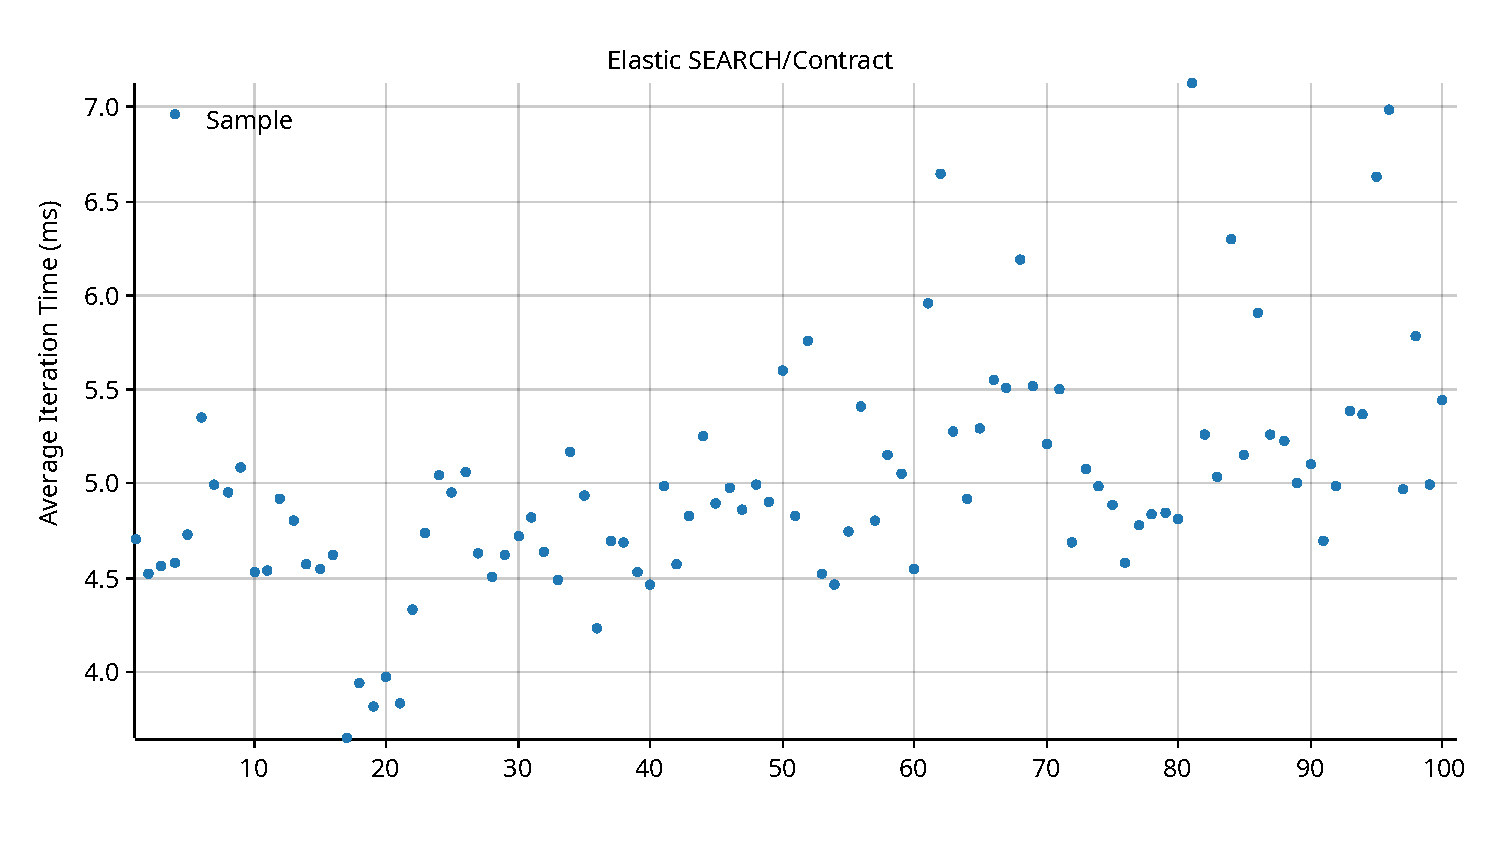
\includegraphics[width=1\linewidth]{images/benchmark/SEARCH/contract/iteration-times.pdf}
	\caption{Diagramma iteration/time richieste \texttt{evaluate} di tipo SEARCH}\label{iter-time contract search}
\end{figure}


%%%%%%%%%%%%%%%%%%%%%%%%%%%%%%%%%%%%%%%%%%%%%%%%%%%%%%%%%%%%
%%%%%%%%%%%%%%%%%%%%%%%%%%%%%%%%%%%%%%%%%%%%%%%%%%%%%%%%%%%%
\section{SQL Benchmark}
Benchmark condotto sulle funzioni \texttt{measure()} ed \texttt{evaluate()} utilizzando la Query SQL descritta nel Codice \ref{JSON query sql} che estrae due campi dall'indice filtrando sulla data.

\paragraph{Confronto funzioni benchate}
La Figura \ref{violino sql} illustra due distribuzioni di probabilità relative al tempo medio di esecuzione delle funzioni \texttt{evaluate} e \texttt{measure}.
Come nel precedente diagramma a violino, sull'asse delle ascisse è presente il tempo di esecuzione mentre su quello delle ordinate i due benchmark da confrontare.
Si può notare come le distribuzioni si concentrino introno al valore medio, 8.5 ms per le metriche e 7.6 ms per i contratti.
Si nota anche come l'ampiezza di entrambi i benchmark, ma prevalentemente di quello Metric, si discosti dal valore medio a causa di alcuni \textit{outliers} misurati, identificati ancora da una riga orizzontale che ne definisce una probabilità irrisoria.
Per concludere, l'esecuzione del benchmark sui contratti è ancora una volta stabile in quanto tutte le misurazioni hanno ottenuto valori addensati intorno ai 7.6 ms, ad eccezione di lievi outlier. 
Il benchmark sulle metriche, come osservato nei benchmark SEARCH, mostra una media leggermente più alta, intorno agli 8.5 ms, a causa di misurazioni outliers più frequenti.
\begin{figure}[H]
	\centering
	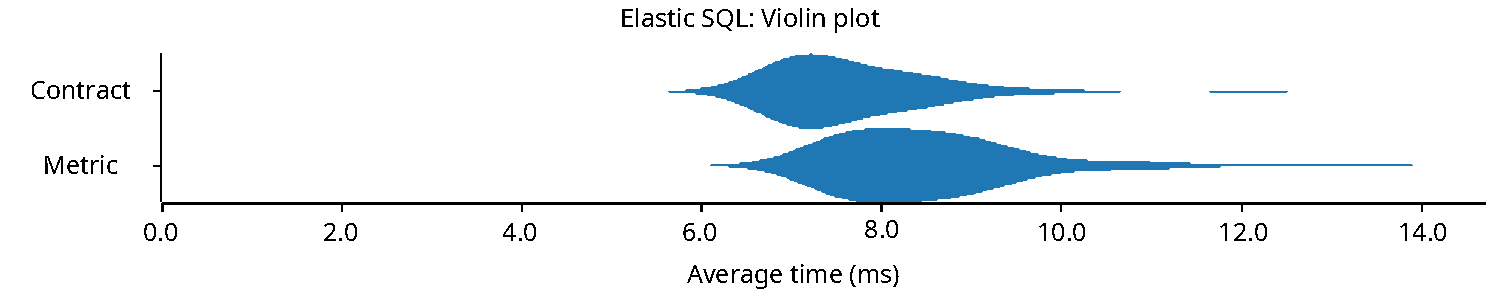
\includegraphics[width=1\linewidth]{images/benchmark/SQL/sql-violin.pdf}
	\caption{Diagramma a violino richieste di tipo SQL}\label{violino sql}
\end{figure}

%%%%%%%%%%%%%%%%%%%%%%%%%%%%%%%%%%%%%%%%%%%%%%%%%%%%%%%%%%%%
%%%%%%%%%%%%%%%%%%%%%%%%%%%%%%%%%%%%%%%%%%%%%%%%%%%%%%%%%%%%
\subsection{Metric - \texttt{measure()}}\label{section metric sql}
\paragraph{Diagramma distribuzione probabilità-tempo}
La Figura \ref{densità metric sql} mostra la distribuzione di probabilità sulle tempistiche di esecuzione del metodo \texttt{measure}.
Si evidenzia anche qui la presenza di un unico picco centrale, che si allontana leggermente dalla media di 8.5 ms a causa della presenza di lievi outliers, al di sopra dei 10.8 ms, che influiscono lievemente sulla valutazione complessiva.
La maggior parte dei dati è concentrata tra 7 e 10 ms.

\begin{figure}[H]
	\centering
	
\includegraphics[width=1\linewidth]{images/benchmark/SQL/metric/density.pdf}
	\caption{Diagramma densità probabilistica richieste \texttt{measure} di tipo SQL}\label{densità metric sql}
\end{figure}

\paragraph{Statistiche calcolate}
Nella Tabella \ref{benchmark sql metric} sono elencate le statistiche ottenute tramite i benchmark, con una media del tempo di esecuzione pari a 8.5 ms e una deviazione standard rispetto tale valore pari a 1.07 ms.
\begin{table}[ht!]
	\caption{Valutazioni statistiche SQL/Metric benchmark}\label{benchmark sql metric}
	\centering
	\begin{tabularx} {0.9\textwidth}
		{C| c*{3}{C}} % C è un column type definito nel main
		\toprule
		\textbf{Misurazione} & \textit{Lower bound} & \textbf{Estimate}  & \textit{Upper bound} \\

		\midrule
		\textbf{Mean}        & 8.3206 ms            & \textbf{8.5206 ms} & 8.7393 ms            \\
		\textbf{Std. Dev.}   & 812.45 µs            & \textbf{1.0723 ms} & 1.3265 ms            \\
		\textbf{Median}      & 8.0902 ms            & \textbf{8.3803 ms} & 8.6017 ms            \\
		\textbf{\gls{MAD}}   & 737.19 µs            & \textbf{895.16 µs} & 1.1394 ms            \\
		\textbf{R2}          & 0.0040924            & \textbf{0.0042356} & 0.0040656            \\

		\bottomrule
	\end{tabularx}
\end{table}

\paragraph{Diagramma Sample-Time}
La Figura \ref{iter-time metric sql} presenta un diagramma che raffigura i tempi di esecuzione della funzione per ciascun sample. Tra i 100 sample presenti non emerge nessuna dispersione significativa nelle valutazioni; sono presenti 5 outlier al di sopra del 10.8. Si evidenzia come la maggior parte dei valori è concentrata nell'intervallo temporale 7 e 10.
\begin{figure}[H]
	\centering
	
\includegraphics[width=1\linewidth]{images/benchmark/SQL/metric/iteration-times.pdf}
	\caption{Diagramma iteration/time richieste \texttt{measure} di tipo SQL}\label{iter-time metric sql}
\end{figure}

%%%%%%%%%%%%%%%%%%%%%%%%%%%%%%%%%%%%%%%%%%%%%%%%%%%%%%%%%%%%
%%%%%%%%%%%%%%%%%%%%%%%%%%%%%%%%%%%%%%%%%%%%%%%%%%%%%%%%%%%%
\subsection{Contract - \texttt{evaluate()}}\label{section contract sql}
\paragraph{Diagramma distribuzione probabilità-tempo}
La Figura \ref{densità contract sql} rappresenta la distribuzione di probabilità del tempo richiesto per l'esecuzione del metodo \texttt{evaluate}.
Si osserva un unico picco centrale che si discosta leggermente dalla media, il cui valore è 7.6 ms. 
Questa variazione è ancora una volta influenzata dalla presenza di outliers sopra i 9.8 ms, che seppur presenti in minima frequenza hanno un impatto sulla valutazione finale.
La concentrazione principale dei valori si colloca tra 6.5 e 9 ms; si notano anche i due valori outlier al di sopra dei 10 ms.
\begin{figure}[H]
	\centering
	
\includegraphics[width=1\linewidth]{images/benchmark/SQL/contract/density.pdf}
	\caption{Diagramma densità probabilistica richieste \texttt{evaluate} di tipo SQL}\label{densità contract sql}
\end{figure}

\paragraph{Statistiche calcolate}
La Tabella \ref{benchmark sql contract} mostra i risultati statistici dei benchmark effettuati, i quali mostrano una media del tempo di esecuzione pari a 7.6 ms e una deviazione standard rispetto tale valore pari a 882.01 µs.
\begin{table}[ht!]
	\caption{Valutazioni statistiche SQL/Contract benchmark}\label{benchmark sql contract}
	\centering
	\begin{tabularx} {0.9\textwidth}
		{C| c*{3}{C}} % C è un column type definito nel main
		\toprule
		\textbf{Misurazione} & \textit{Lower bound} & \textbf{Estimate}  & \textit{Upper bound} \\

		\midrule
		\textbf{Mean}        & 7.4923 ms            & \textbf{7.6578 ms} & 7.8354 ms            \\
		\textbf{Std. Dev.}   & 666.71 µs            & \textbf{882.01 µs} & 1.1105 ms            \\
		\textbf{Median}      & 7.3017 ms            & \textbf{7.4661 ms} & 7.6194 ms            \\
		\textbf{\gls{MAD}}   & 505.58 µs            & \textbf{729.81 µs} & 898.74 µs            \\
		\textbf{R2}          & 0.0102391            & \textbf{0.0105995} & 0.0101868            \\

		\bottomrule
	\end{tabularx}
\end{table}

\paragraph{Diagramma Sample-Time}
Nella Figura \ref{iter-time contract sql} viene raffigurato un diagramma che rappresenta il tempo di esecuzione di ciascun sample per terminare la funzione. 
Su 100 sample presenti, di cui l'altezza ne indica il tempo impiegato, non si nota nessuna dispersione significativa nelle valutazioni.
\'E il benchmark con il minor numero di outlier, solo 2 sono presenti sopra al valore 9.8. I valori si condensano tutti nell'intervallo temporale 6.5 e 9.

\begin{figure}[H]
	\centering
	
\includegraphics[width=1\linewidth]{images/benchmark/SQL/contract/iteration-times.pdf}
	\caption{Diagramma iteration/time richieste \texttt{evaluate} di tipo SQL}\label{iter-time contract sql}
\end{figure}
%%%%%%%%%%%%%%%%%%%%%%%%%%%%%%%%%%%%%%%%%%%%%%%%%%%%%%%%%%%%
%%%%%%%%%%%%%%%%%%%%%%%%%%%%%%%%%%%%%%%%%%%%%%%%%%%%%%%%%%%%






